\documentclass[12pt,letterpaper]{article}
\usepackage[top=2cm,left=2cm,right=2cm,bottom=2cm]{geometry}
\usepackage[utf8]{inputenc}
\usepackage[T1]{fontenc}  
\usepackage{ae}
\usepackage{amsmath,amssymb}
\usepackage{setspace}
\usepackage{graphicx}
\usepackage{indentfirst}
\usepackage{url}
\usepackage{color}
\usepackage{cite}
\usepackage{gensymb}
\usepackage{subcaption}
\usepackage{hyperref}
\usepackage{epigraph}
\usepackage{mathtools}
\usepackage{mathrsfs}
\usepackage{epstopdf}

\definecolor{red}{rgb}{1.0,0.0,0.0}
\definecolor{green}{rgb}{0.01,0.75,0.24}
\definecolor{blue}{rgb}{0.0,0.0,1.0}

\newcommand{\ket}[1]{| #1 \rangle}
\newcommand{\bra}[1]{\langle #1 |}
\newcommand{\expected}[1]{ \langle #1 \rangle}
\newcommand{\product}[2]{\langle #1 | #2 \rangle}
\newcommand{\pib}{\boldsymbol{\pi}}
\newcommand{\sigmab}{\boldsymbol{\sigma}}
\newcommand{\bvec}[1]{\boldsymbol {#1}}
\newcommand{\project}{\large Research Project Renewal  \vskip 0.1cm}
\newcommand{\asu}{Physics Department \\ Arizona State University}

\begin{document}
\onehalfspacing
%\doublespace
\title{\project {\Large \textbf{Quantum Monte Carlo Calculations of Nucleon 
Systems and Cold Atom Gases}} \vspace{0cm}}
\author{
{\bf PIs: Kevin E. Schmidt}, Arizona State University \\
{\bf Stefano Gandolfi}, Los Alamos National Laboratory
}
\date{\today}
\maketitle

\vspace*{-2.0cm}

\section*{Abstract}

This research project renewal request is for 50,000 SUs on Stampede2.
We describe our progress on cold atom gases simulations and nucleon systems 
calculations.
We propose a project related to strongly-interacting Fermi gas systems.
We present our progress on explicitly including the pionic degrees of 
freedom in 
the nuclear Monte Carlo simulations, and we introduce the next steps,
related to larger nuclei.
We also have been developing improved trial wave functions for nuclei and 
nuclear matter, and we intend to continue our research by extending these wave 
functions to other nucleon systems.
In summary, we will continue to employ
Quantum Monte Carlo methods to study nucleon systems and cold atom gases, by 
using  
our large-scale highly-parallel code, which 
has been successfully used to calculate properties of cold gases, nuclear 
matter, 
neutron matter, and medium-mass nuclei.

\section{Research Objectives}

This allocation renewal request is intended to provide the computational 
resources 
to continue to carry out the project \textit{Quantum Monte Carlo (QMC) 
Calculations of 
Nucleon Systems} supported by the National Science Foundation grant 
PHY-1404405, and related projects.

Many nuclear processes in our universe occur under extreme conditions in 
supernovae and neutron stars. The properties of nuclei and nuclear matter 
under these conditions, which are difficult or impossible to reproduce in 
the laboratory, must necessarily be calculated theoretically. These data are 
needed to understand astrophysically important systems and processes such as 
neutron rich matter, neutron stars, supernovae, and r-process 
nucleosynthesis and neutrino scattering. The quantum many-particle methods 
developed within this project have broad applications across many areas of 
physics, including nuclear physics, cold atomic gas research, and electronic 
structure. Methods 
previously developed within this project have been applied in each of these 
areas.

The results of this project are relevant for the nuclear physics program at 
the Department of Energy Office of Science, that has identified the 
knowledge of the structure of nuclei and nuclear matter as one of the most 
important scientific questions in nuclear physics in the most recent Nuclear 
Science Advisory Committee long-range plan.

In this document we summarize the advances we have achieved, in addition 
to the proposed plan for the current cycle.
In Sec.~\ref{sec:cold} we describe an interesting project involving
cold atomic Fermi gases.
The inclusion of explicit pion field contributions in simulations of nucleon 
systems is discussed in Sec.~\ref{sec:pions}.
In Sec.~\ref{sec:improved} we present our study of improved wave functions for 
nuclei and nuclear matter.

\subsection{Three-component Fermi gas}
\label{sec:cold}

There are three relevant length scales in an attractive two-component Fermi gas: the effective range of
the potential $r_e$, the s-wave scattering length $a$, and $n^{-1/3}$ the
interparticle distance ($n$ being the number density). The diluteness condition
corresponds to $n^{-1/3} \gg r_e$, while the BEC scheme coincides with
$1/(na^3)\gg 1$, and the BCS scheme $1/(na^3)\ll -1$.
At the heart of the
BEC-BCS crossover there is the unitary regime, $1/(na^3)=0$, which
is a strongly
interacting system with short-range interactions of remarkable
properties.  

In a three-component Fermi gas there are two more main ingredients: the competition between pairing and binding among different atom pairs, and
the role of three-body correlations.
The Thomas
effect (the collapse of the three-body system as $r_e$ $\to$ 0 at fixed $a$) and the Efimov effect (the
accumulation of three-body bound states at threshold as a$\to\infty$ at fixed $r_e$) are consequences of the
strong attraction among three resonating particles. These can occur
only if the three particles in the system can overlap in space, which is forbidden by the Pauli exclusion principle in the case of only two species.

At zero temperature, the properties of
the system depend on 4 parameters: the three scattering lengths ($a_{12}$, $a_{13}$, $a_{23}$) and the three-body parameter. The authors in
Ref.~\cite{bed09} used qualitative arguments and found a rich phase diagram
for this system.
There were several reports of experimental realizations of a three-component
$^6$Li gas. One of them attributed 
enhanced three-body recombination in the gas to an excited Efimov trimer state
\cite{wil09}.
Another work studied the atom loss in a
mixture of atoms and dimers, and found two peaks corresponding to the degeneracy points of the energy levels of the dimers and the ground- and first-excited Efimov trimers \cite{nak10}.

Our objective with this project is to determine properties (such as phase diagrams, equations of state, and pairing gaps) of a dilute gas with three
fermionic species at zero temperature. We will employ variational and
diffusion Monte Carlo methods to determine properties of these systems.
These are many-body methods that have been
successfully used by us to calculate properties of strongly-interacting
fermionic systems \cite{mad16,mad17,mad18,madeira19} using
XSEDE resources.

\subsection{QMC simulations with explicit contributions from the pion field}
\label{sec:pions}

In most simulations of nonrelativistic nuclear systems, the wave functions found solving
the many-body Schr\"odinger equations describe the quantum-mechanical amplitudes of
the nucleonic degrees of freedom. In those simulations the pionic contributions are
encoded in nuclear potentials and electroweak currents, and they determine
the low-momentum behavior. In Ref.~\cite{mad18} we presented a novel quantum Monte Carlo formalism in
which both relativistic pions and nonrelativistic nucleons are explicitly included in the quantum-mechanical 
states of the system.
We started from the
heavy baryon leading order chiral Lagrangian density in which only nucleon and pion degrees of freedom are included,
\begin{eqnarray}
\mathcal{L}_0 &=
\frac{1}{2}\partial_\mu \pi_i \partial^\mu \pi_i
- \frac{1}{2} m_\pi^2 \pi_i \pi_i + N^\dagger \Big[ i\partial_0 +\frac{\nabla^2}{2M_0}
- \frac{1}{4f_\pi^2}\epsilon_{ijk} \tau_i \pi_j \partial_0\pi_k 
-\frac{g_A}{2f_\pi} \tau_i \sigma^j \partial_j \pi_i
-M_0\Big] N\nonumber \\
&
-\frac{1}{2} C_S(N^\dagger N) (N^\dagger N)
-\frac{1}{2} C_T (N^\dagger \sigma_i N) (N^\dagger \sigma_i N)\, ,
\label{eq:L_0}
\end{eqnarray}
where $m_\pi$ is the pion mass,
$M_0$ is the bare nucleon mass,
$f_\pi=$ 92 MeV is the pion decay constant,
$g_A=1.26$ is the nucleon axial-vector coupling constant, $C_S$ and $C_T$ are low-energy constants, and $i = x, y, z$. We derived the
Hamiltonians for a system composed of $A$ nucleons and pions,
\begin{eqnarray}
\label{eq:hqmc}
H&=&H_N+H_{\pi\pi}+H_{AV}+H_{WT},
\nonumber\\
H_N &=& \sum_{i=1}^A \left [ \frac{P_i^2}{2M_P}+M_P
+\beta_K P_i^2 + \delta M\right ]
+\sum_{i<j}^A \delta_{R_0}(\bvec r_i-\bvec r_j)
[C_s+C_T\bvec \sigma_i\cdot \bvec \sigma_j ],
\nonumber\\
H_{\pi\pi} &=& \frac{1}{2}{\sum_{\bvec k}}' \left [
|\bvec \Pi^c_{\bvec k}|^2+
\omega_{\bvec k}^2
|\bvec \pi^c_{\bvec k}|^2
+|\bvec \Pi^s_{\bvec k}|^2+
\omega_{\bvec k}^2
|\bvec \pi^s_{\bvec k}|^2
\right ],
\nonumber\\
H_{AV} &=&
\sum_{i=1}^A
\frac{g_A}{2 f_\pi} \sqrt{\frac{2}{L^3}}
{\sum_{\bvec k}}^\prime \left\{\bvec \sigma_i \cdot \bvec k
\left[\bvec \tau_i \cdot \bvec \pi_{\bvec k}^s \cos(\bvec k \cdot \bvec r_i)
-  \bvec \tau_i\cdot \bvec \pi_{\bvec{k}}^c
\sin(\bvec k \cdot \bvec r_i)\right]\right\},
\nonumber\\
H_{WT} &=&\sum_{i=1}^A
\frac{1}{2f_\pi^2 L^3} \bvec \tau_i
\cdot \left [
\rule[-1.1em]{0em}{0em}
\right .
{\sum_{\bvec k}}' \cos(\bvec k \cdot \bvec r_i) \bvec \pi^c_{\bvec k}
\times
{\sum_{\bvec q}}' \cos(\bvec q \cdot \bvec r_i) \bvec \Pi^c_{\bvec q}
\nonumber\\
&+&
{\sum_{\bvec k}}' \cos(\bvec k \cdot \bvec r_i) \bvec \pi^c_{\bvec k}
\times
{\sum_{\bvec q}}' \sin(\bvec q \cdot \bvec r_i) \bvec \Pi^s_{\bvec q}
+
{\sum_{\bvec k}}' \sin(\bvec k \cdot \bvec r_i) \bvec \pi^s_{\bvec k}
\times
{\sum_{\bvec q}}' \cos(\bvec q \cdot \bvec r_i) \bvec \Pi^c_{\bvec q}
\nonumber\\
&+& \left .
{\sum_{\bvec k}}' \sin(\bvec k \cdot \bvec r_i) \bvec \pi^s_{\bvec k}
\times
{\sum_{\bvec q}}' \sin(\bvec q \cdot \bvec r_i) \bvec \Pi^s_{\bvec q}
\right ].
\end{eqnarray}
Instead of complex amplitudes for the pion fields, we worked with
real amplitudes for the sine/cosine modes, hence $\bvec \pi_{\bvec k}^{c,s}$
denotes the component with momentum $\bvec k$ of the field, and the $\bvec \Pi_{\bvec k}^{c,s}$ are the conjugate momenta.
$\beta_K$ and $\delta M$ are counter terms,
introduced due to our cutoff.
The $\delta_{R_0}$ function is a smeared off contact used for two-body
interactions. The subscript ``AV'' refers to the pion-nucleon axial-vector coupling, whereas ``WT'' stands for the Weinberg-Tomozawa tadpole term.

We built the wave functions for $A$ nucleons,
\begin{align}
\label{eq:psitqmc}
&\langle RS\Pi|\Psi_T\rangle =
\langle RS\Pi|
\exp\left\{
-{\sum_{\bvec k}}^\prime \left [
\frac{\omega_k}{2}(
|\bvec{\pi}_{\bvec{k}}^c|^2
+|\bvec {\pi}_{\bvec{k}}^s|^2)
+\frac{\alpha_k}{2\omega_k}
\left (
\bvec \pi_{\bvec k}^c \cdot \bvec B^c_{\bvec k}
+\bvec \pi_{\bvec k}^s \cdot \bvec B^s_{\bvec k}
\right )\right.\right.
\nonumber\\
&
\left .
\left .
-\frac{1}{4}\omega_k\alpha_k^2 G_k^2 \sum_{i<j}^A
\bvec \tau_i\cdot\bvec \tau_j
\bvec\sigma_i\cdot \bvec k
\bvec\sigma_j\cdot \bvec k
\cos(\bvec k\cdot \bvec r_{ij})
\right] \right \}
|\Phi\rangle\, ,
\end{align}
where $R$ stands for all nucleon positions and $S$ for the spin-isospin
degrees of freedom, and $\Pi$ for all pion amplitudes. The other
quantities and the rationale behind this choice of wave function
are given in Ref.~\cite{mad18}. We used Eqs.(\ref{eq:hqmc}) and (\ref{eq:psitqmc}), together with QMC methods, to calculate
the renormalization of the nucleon mass
as a function of the momentum cutoff, a Euclidean time density
correlation function that deals with the short-time nucleon diffusion, and the pion cloud density and
momentum distributions. In the two nucleon sector we showed that the interaction of two static nucleons
at large distances reduces to the one-pion exchange potential, and we fit the low-energy constants of the
contact interactions to reproduce the binding energy of the deuteron and two neutrons in finite volumes.

Currently we are 
applying this method to light-nuclei, the triton and the alpha particle, $A=3$ and 4.
We found evidences that these systems are overbound, even for
relatively small cutoffs. Currently, we are investigating the source
of this overbinding, and possible ways of circumventing it.

\subsection{Improved trial wave functions for nuclei and nuclear matter}
\label{sec:improved}

{\color{red} copied and pasted}

In QMC calculations, the results are dependent on the accuracy of the trial wave function employed
to constrain the path to control the fermion sign problem.
The statistical errors also can be reduced with accurate trial functions.
We have recently introduced a linearly pair-correlated wave function which has greatly improved the convergence of our results \cite{gan14}. We are now working on including multiple pair correlations to study their effect. We have written codes to efficiently handle the large number of matrix operations required to include these additional correlations.

We have been able to add quadratic correlations to the trial wave function that we use in nuclear Monte Carlo calculations. These additional correlations have caused the energies to decrease for the nuclei $^4$He and $^{16}$O, as well as for symmetric nuclear matter. The quadratic correlations resulted in an improved trial wave function, but were too expensive to use on larger nuclear systems. Our results for this wave function have been submitted for review to the Physical Review C journal \cite{lon18}. Linear and quadratic correlations come from an expansion of the exponential correlation. We have begun to include the full set of exponential correlations in the nuclear trial wave function
by sampling the terms,
and significant progress has been made. We expect to be doing full production runs with this trial wave function shortly.

We then plan to use these improved wave functions to investigate the clustering of nucleons into alpha particles in mostly neutron matter. We intend to study the convergence of variational and auxiliary field diffusion Monte Carlo with these new wave functions for nuclei and nuclear matter with up to $A=40$.

\section{Computational Methods}
\label{sec:comp_met}

We use QMC methods, in particular Auxiliary Field Diffusion Monte Carlo 
(AFDMC) methods, which have proven to be very successful in calculating 
ground-state properties including momentum distributions, as we have shown 
in our article for Reviews of Modern Physics \cite{car15}. The AFDMC code 
has been successfully used to calculate properties of nuclear matter, 
neutron matter, and medium-mass nuclei \cite{gan14}. The results of 
Ref.~\cite{gan12} showed the relation between the symmetry energy and 
properties 
of neutron stars.

We have written a large-scale highly-parallel code to achieve high precision 
calculations for many properties of medium-mass nuclei. The AFDMC code 
calculates the
ground-state of the nucleus through a branching random walk algorithm, and it
can be used to compute other properties including radii and momentum 
distributions.

\subsection{Algorithm and implementation}

The AFDMC code has been developed by the investigators of this project. The 
AFDMC method is used to extract the ground-state component of the system 
from the variational ansatz describing the system. This is done with a 
projection in imaginary-time, i.e. we calculate
\begin{equation}
\label{eq:dif}
\lim_{n\rightarrow\infty}\left[ e^{-H\delta\tau}\right]^n \Psi_T(R,S) 
\rightarrow \Psi_0(R',S'),
\end{equation}
where $R =(r_1, \cdots, r_N)$ are the coordinates of nucleons, $S = (s_1, 
\cdots, s_N)$ are complex numbers indicating their spin and isospin 
projections, and $\Psi_T(R,S)$ is a trial variational wave function. The 
algorithm is a branching random walk that requires the diagonalization of 
$3N \times 3N$ matrices ($N$ is the number of particles) at each step of the 
random walk. AFDMC is written in Fortran2008 and MPI, and it uses the vendor 
optimized BLAS and LAPACK libraries to perform matrix diagonalizations at 
each step.

The AFDMC algorithm is a variant of Diffusion Monte Carlo, where each step 
involves:
\begin{enumerate}
\item Diffuse nucleon’s positions, $R \rightarrow R'$ according to the 
kinetic energy $T$ of the Hamiltonian.
\item Rotate nucleon’s spins, $S \rightarrow S'$, according to the spin and 
isospin-dependent potential.
\item Calculate the weight $W$ of the new configuration, and generate $n$ 
replicas of the new configuration according to $n = [W + \eta]$, where 
$\eta$  is a random number uniformly distributed from 0 to 1.
\end{enumerate}

This algorithm is implemented by considering
a collection of configurations (called \textit{walkers})
that are simultaneously evolved in imaginary-time. The parallelization is 
accomplished
by spreading the configurations among the nodes. However, AFDMC is not quite
embarrassingly parallel because the branching term generates fluctuations in 
the number of configurations, of the order up to 10\%, and the calculation 
of observables requires an average over walkers at the same imaginary-time. 
We employ a dynamic load rebalancing after
each time step to redistribute walkers across nodes.

\section{Application efficiencies}

We describe in detail the 
performance and scaling of our code in the additional document submitted 
with this proposal. The most relevant feature that we present in that 
document is the scaling in XSEDE resources, namely Stampede2 and SuperMIC.
We tested the 
performance of the code on Stampede2. Up to
{\color{red} 4096 ???}
cores, the 
largest number tested, the code scales strongly, Fig.~\ref{fig:stampede}.
We also verified that our code
scales strongly on SuperMIC, Fig.~\ref{fig:supermic}, up to 2560 cores (the 
largest number tested).

\begin{figure}[!htb]
\centering
\begin{subfigure}{.45\textwidth}
  \centering
  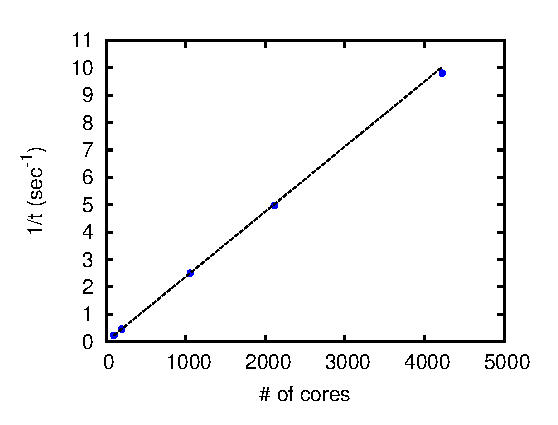
\includegraphics[width=\textwidth]{stampede.eps}
  \caption{}
  \label{fig:stampede}
\end{subfigure}%
\hspace{0.01\textwidth}
\begin{subfigure}{.45\textwidth}
  \centering
  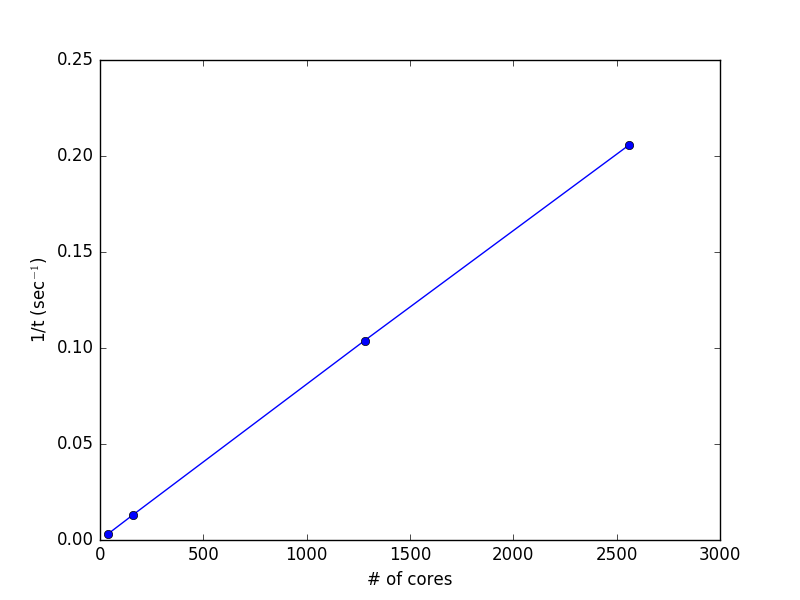
\includegraphics[width=\textwidth]{supermic.png}
  \caption{}
  \label{fig:supermic}
\end{subfigure}
\caption{Scaling on Stampede2 (a) and SuperMIC (b) using the time to propagate 
10000 configurations of an $^{16}$O nucleus for 100 steps.}
\label{fig:scaling}
\end{figure}

\section{Computational Research Plan and Justification for Requested 
Resources}

As discussed in Sec. \ref{sec:comp_met}, the simulations depend on a trial 
variational wave function. The variational parameters are determined using 
the stochastic reconfiguration method \cite{cas04}
and the linear method \cite{con17}. Once these parameters 
are determined, we can proceed with the computation of physical quantities 
of interest. We base our estimates on the amount of SUs and storage used in 
\cite{car15} 
and references therein.

\subsection{Three-component Fermi gases}

We wish to perform simulations for a wide range of systems.
Let us denote each component by A, B and C, and $N_A$, $N_B$, and
$N_C$ the respective number of particles of each component. We wish
to investigate the cases: $N_A=N_B=N_C$, equal populations; and
$N_A=N_B$ and $N_C=1$, the polaron problem. The interactions
between components can be varied, and the atomic mass of each component
can be different as well. This gives rise to several cases that need
to be simulated.

We estimate 1,000 SUs for code development, 
5,000 SUs for the variational optimization of the parameters, 
and 11,000 SUs for production runs.

\subsection{QMC simulations with explicit contributions from the pion field}

We want to perform simulations with different system 
sizes, ranging from three nucleons plus the pion field up to four nucleons plus 
the pion field. Several runs are needed for each 
system, because we have to investigate the behavior of properties as a function 
of the box size and number of pion modes, for example.

We require approximately 1,000 SUs for code development and
5,000 SUs for the variational optimization of the parameters. 
Longer runs are necessary to compute quantities
such as energy of the system, density and other distribution functions, 
with small variances. We estimate 11,000 SUs for these computations.
 

\subsection{Improved QMC simulations for nuclei and nuclear matter}

{\color{red} recalculate}

We want to do energy calculations on three systems, $^4$He, $^{16}$O, and
symmetric nuclear matter using the new exponential correlations to compare the
trial wave function with the linear and quadratic correlations. To do this we
will need to optimize a new set of parameters. We estimate that this will
require 2,000 SUs for development, 4,000 SUs to optimize the variational
parameters for the new correlations, and 18,000 SUs to calculate the energies
for the three nuclear systems mentioned above.

With this improved wave function we will be investigating the clustering of
alpha particles in mostly neutron matter. We will be doing calculations for a
variety of densities to investigate the clustering dependence on density. We
estimate that this will require 2,000 SUs for development, 4,000 SUs to
optimize the code for mostly neutron matter, and 18,000 SUs to calculate the
clustering at a variety of densities.

\subsection{Summary of the requested resources}

We present in Table \ref{tab:SUs} the amount of SUs requested for each task.
We are requesting a total of 50,000 SUs on Stampede2.
We also included SUs for the code 
development, in order to ensure performance and scaling during execution.
As for storage needs, we request the default value of 5 GB per user. The size 
of input, 
output and configuration files is of approximately 50 MB per system. As the 
simulations are independent, there is no need to store all of them at the 
same time at Stampede2. We are capable of handling the post-processing of the 
simulations in our local computing environments.

\begin{table}[htbp]
\caption{Justification for the requested amount of SUs}
\begin{tabular}{|l|r|r|r|}
\hline
 & \textbf{Fermi gases} & \textbf{Explicit pions} & \textbf{Improved QMC simulations} \\ \hline
Development 			 & 1,000 & 1,000 & 1,000 \\ \hline
Variational optimization & 5,000 & 4,000 & 5,000 \\ \hline
Production 				 &11,000 & 11,000 & 11,000 \\ \hline
Subtotal 				& 17,000 & 16,000 & 17,000 \\ \hline\hline
\multicolumn{4}{|c|}{\textbf{Total: 50,000 SUs}} \\ \hline
\end{tabular}
\label{tab:SUs}
\end{table}


\section{Additional considerations}

We believe that we have enough funding, through the NSF grant, and qualified 
staff to complete the work plan described in this project.

\subsection{Qualifications of the PIs and team}

\textbf{PIs}

\underline{Kevin Schmidt} {\color{red} update}
Kevin Schmidt in collaboration with Stefano Fantoni developed the
auxiliary field diffusion Monte Carlo method. With collaborators
he performed the first diffusion and auxiliary field quantum
Monte Carlo calculations for paired fermions.  He is a fellow of
the American Physical society and has published more than 150 papers.

\underline{Stefano Gandolfi} {\color{red} update} is a nationally and 
internationally recognized scientist in Many-Body Nuclear Theory.
He has published more than 50 papers and he has about 
3,100 citations on Google Scholar. As a result of his excellent work, 
Gandolfi received the International Union of Pure and Applied Physics prize 
for young researchers in nuclear physics in 2013. He has led a program in 
Quantum Monte Carlo at the Institute of Nuclear Theory in 2013, among other
conferences in 2017 and 2018.

\textbf{Post-doctoral researcher}

\underline{Lucas Madeira} is a post-doctoral researcher
at University of São Paulo.
He has several works in collaboration with Kevin Schmidt and Stefano
Gandolfi.
His research interests include strongly interacting fermionic systems, such as 
cold atom gases and nucleon systems.
He has experience with High Performance 
Computing including MPI and OpenMP.

\textbf{Graduate student}

\underline{Cody Petrie} is a PhD student at Arizona State University. He 
received a BS in Physics from Brigham Young University in 2014. He has been 
doing computational nuclear physics for the past four and a half years.

\vspace*{-0.5cm}

\bibliographystyle{unsrt}
\bibliography{xsede}
\end{document}
